\chapter{Adaptierbarkeit}
Das ganze was ich aufgebaut habe soll ja auch für andere Module der Maschine funktionieren. Wie kann man das einfach
machen? Man muss eben ein paar Standards einbauen. Wie können die aussehen? Folgend ein paar Ideen was definiert werden
muss.

- wie müssen die Daten aussehen
- Wie wird das Netz trainiert
- Nutzen für andere Module der Maschine\\ \\

Das Vorgehen: \\
- Daten zusammenstellen
- Daten überprüfen
- Daten in Watson Studio laden
- Daten konvertieren
- Neuronales Netz aufbauen
- Model exportieren
- Dann ein Deployment machen oder TensorFlow
- Schnittstelle ansteuern
- Eventuell API-Connect anpassen
- Angular-Komponente hinzufügen
- Formatvorlage kopieren
- Menüpunkt hinzufügen
- Dateneingabe und die Ausgabe anpassen\\ \\

Das ganze wird an dem Projekt \enquote{Haribo} veranschaulicht.

\begin{figure}[h]
    \centering
    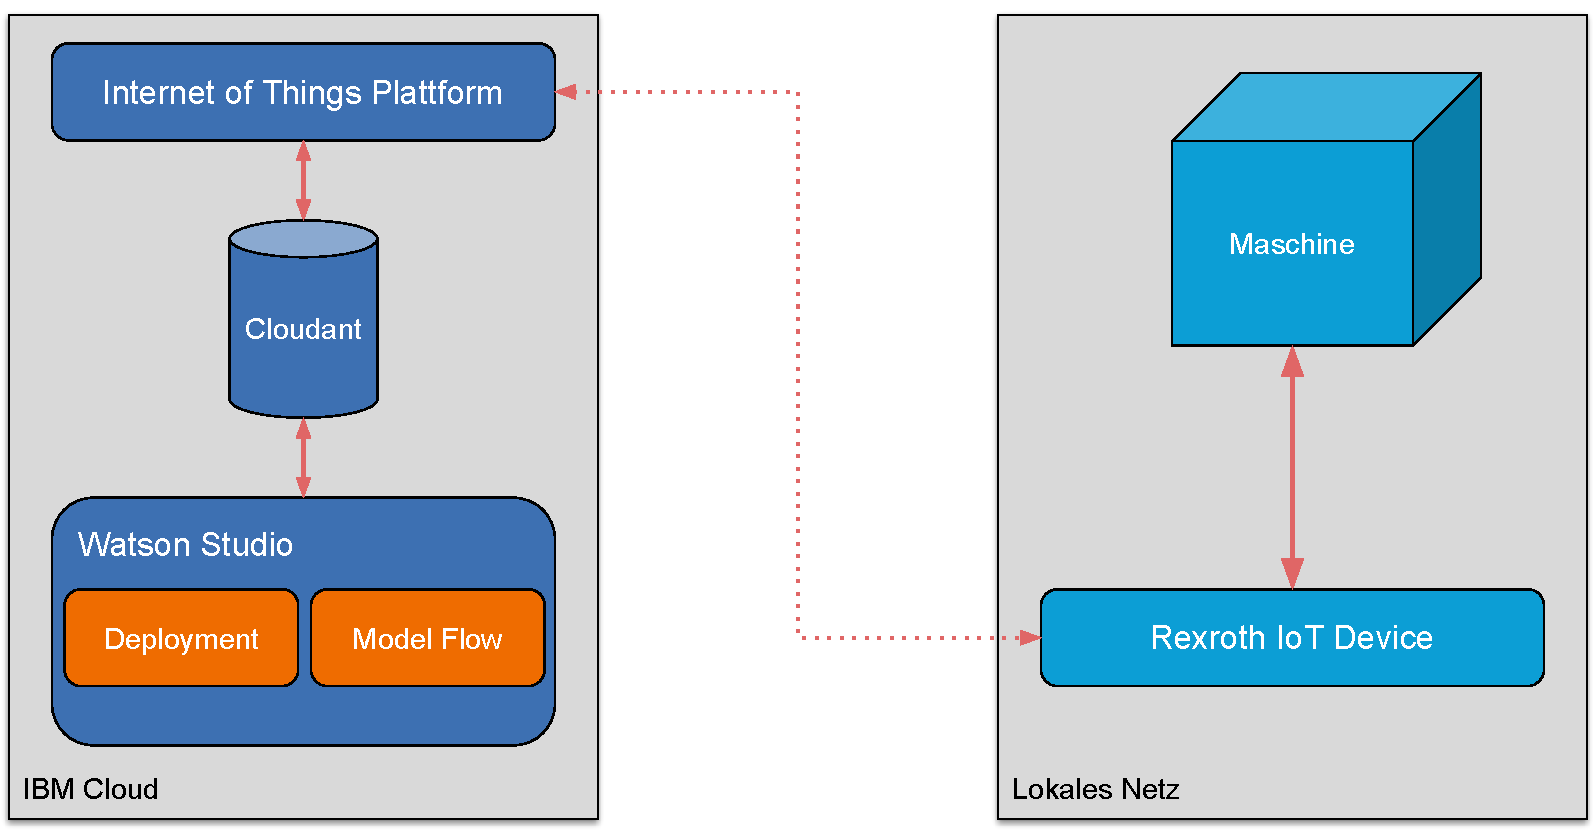
\includegraphics[scale=0.5]{images/kapitel_5/architektur_uebersicht.pdf}
    \caption{Übersicht der Zielarchitektur}
    \label{fig:umsetzung_zielarchitektur_5}
\end{figure}

\colorbox{yellow}{Hier fehlt was}